% saddle_order.tex -- self-contained statement and proof of the main result: the order of the saddles
% visited by gradient flow on tree tensor networks after one component is learned, and the plateau laws.
% Sources: notes/theory_saddle_order.md v2 (verified twice), report App. A.2-A.4, experiments/locality,
% experiments/saddle_dyn. Build: from report/, pdflatex saddle_order; bibtex saddle_order; pdflatex x2.
\documentclass[11pt]{article}
\usepackage[T1]{fontenc}
\usepackage[utf8]{inputenc}
\usepackage{lmodern}
\usepackage[margin=1in]{geometry}
\usepackage{amsmath,amssymb,amsthm}
\usepackage[dvipsnames]{xcolor}
\usepackage{enumitem}
\usepackage{tikz}
\usepackage[round,authoryear]{natbib}
\usepackage[colorlinks=true,linkcolor=MidnightBlue,citecolor=OliveGreen,urlcolor=RoyalPurple]{hyperref}
\setlist{itemsep=2pt,topsep=3pt}
\setlength{\parskip}{3pt}

\newtheorem{theorem}{Theorem}
\newtheorem{proposition}{Proposition}
\newtheorem{lemma}{Lemma}
\newtheorem{corollary}{Corollary}
\theoremstyle{definition}
\newtheorem{definition}{Definition}
\newtheorem{example}{Example}

\newcommand{\St}{\mathrm{St}}
\newcommand{\ord}{\mathrm{ord}}
\newcommand{\ip}[2]{\langle #1,#2\rangle}

\title{The order of saddle points in tree tensor network training}
\author{}
\date{October 2026}

\begin{document}
\maketitle
\vspace{-2.5em}

\begin{abstract}
We study gradient flow on tree tensor networks (TTNs) fitted to a target that is a sum of rank-one
tensors. From small initialization the flow learns the rank-one terms one at a time and stays near a
saddle point between consecutive terms. How long it stays is controlled by the order of the saddle, the
lowest power of the distance at which the loss can decrease. We compute this order exactly at the saddle
reached after one term has been learned. Typically it equals the number of cores in the smallest subtree
that connects the cores on which some unlearned term differs from the learned one. This number depends on
the shape of the tree, so the same target produces plateaus of different lengths on different trees. The
order is lower only when the unlearned terms are, in a precise spectral sense, stronger than the learned
one, and we give its value in that case too. At leading order, a saddle of order $p$ is left after a time
$\propto\ln(1/\sigma)$ if $p=2$ and $\propto\sigma^{-(p-2)}$ if $p\ge3$, where $\sigma$ is the initialization
scale; simulations on nine trees agree.
\end{abstract}

\section{Introduction}

In a deep linear network (DLN) trained from small initialization, gradient flow learns the singular modes
of the target one at a time, with a plateau before each \citep{saxe2014exact,jacot2022saddletosaddle}. Every
plateau lasts $\propto\sigma^{-(K-2)}$, where $K$ is the depth and $\sigma$ the initialization scale. The reason is
that the output is a product of $K$ layers that all start at size $\sigma$: their common size $a$ obeys
$\dot a\approx c\,a^{K-1}$, whose solution from $a(0)=\sigma$ stays small for a time $\propto\sigma^{-(K-2)}$ and then
grows quickly. In a DLN every mode needs every layer, so every plateau has the same exponent.

A TTN is also a product of $K$ factors, its cores, but each core is attached to only some of the inputs. After
the first term is learned, most cores are large. To add the next term, only some cores need to change from
small values, and the length of the next plateau depends on how many. In the language of the loss landscape,
it depends on the order of the saddle at which the flow rests.

This note determines that order (Theorem~\ref{thm:main}) and derives the resulting plateau lengths
(Proposition~\ref{prop:escape}). Section~\ref{sec:prior} compares the result with prior work.

\section{Setting and definitions}\label{sec:setting}

\paragraph{Tree tensor networks.} Let $T$ be a tree with $K$ nodes. Each node $v$ holds a tensor $G_v$, called a
\emph{core}. A core has one leg for each tree edge at $v$ and, possibly, one \emph{physical} leg of dimension
$D_v$. The legs on a tree edge $e$ have dimension $\chi_e$, the \emph{bond dimension}. Contracting all
tree-edge legs gives a tensor $W(\theta)\in\bigotimes_v\mathbb R^{D_v}$, where $\theta$ denotes all core entries.
The network has $N$ inputs $x_0,\dots,x_{N-1}\in\mathbb R^d$, called \emph{sites}; each site belongs to the physical leg
of one core, so $D_v=d^{n_v}$ if core $v$ carries $n_v$ sites ($D_v=1$ if it carries none). The network computes
$f(x)=\ip{W}{x_0\otimes\dots\otimes x_{N-1}}$.

Three trees serve as examples (Figure~\ref{fig:steiner}): the matrix product state (MPS), a path with one site
per core; the binary tree, with two sites on each bottom core and none on the others; and the hierarchical
Tucker (HT) tree, with one site on each leaf and none on the internal cores.

\paragraph{Target and loss.} Labels are generated by a target tensor $W^*$ as $y=\ip{W^*}{x_0\otimes\dots\otimes x_{N-1}}$.
For whitened Gaussian inputs the population squared loss is, up to a constant,
\begin{equation}
L(\theta)=\tfrac12\lVert W(\theta)-W^*\rVert^2 .
\end{equation}
We take $W^*$ to be a sum of distinct products of standard basis vectors,
\begin{equation}\label{eq:target}
W^*=\sum_{r}s_r\,U_r,\qquad U_r=e_{\pi_r(0)}\otimes e_{\pi_r(1)}\otimes\dots\otimes e_{\pi_r(N-1)},\qquad s_r>0,
\end{equation}
where $\pi_r$ is a string of basis indices, one per site (for example $\pi_r=110010$). We call $U_r$ the
\emph{components} of the target. Distinct components are orthonormal.

\paragraph{The saddle after one component is learned.} Fix a component $j$ and let $q_v\in\mathbb R^{D_v}$ be the
basis vector that $U_j$ has on the sites of core $v$, so $U_j=\bigotimes_vq_v$. The point $\theta_S$ has cores
\begin{equation}\label{eq:saddle}
G_v=a_v\;q_v\otimes e_0\otimes\dots\otimes e_0,\qquad \textstyle\prod_va_v=s_j,
\end{equation}
where $e_0$ is the first basis vector of each tree-edge leg. Then $W(\theta_S)=s_jU_j$: the network represents
component $j$ exactly, using one channel (index $0$) on every edge. Every critical point with $W=s_jU_j$ has this
form after a change of basis on the edges. The other $\chi_e-1$ indices of each edge are \emph{unused channels}.
The loss at $\theta_S$ is $L_S=\frac12\lVert\mathcal R\rVert^2$, with residual $\mathcal R=W^*-s_jU_j=\sum_{r\ne j}s_rU_r$.

\paragraph{Order of a saddle.} The order of a critical point $\theta_S$ is the largest $p$ such that, for some
$C>0$,
\begin{equation}\label{eq:order}
L(\theta)-L_S\ \ge\ -C\,\lVert\theta-\theta_S\rVert^{p}\qquad\text{for all $\theta$ near $\theta_S$.}
\end{equation}
Equivalently, it is the smallest $p$ for which some curve with $\lVert\theta(t)-\theta_S\rVert\le t$ has
$L(\theta(t))-L_S\le-ct^p$ ($L$ is a polynomial, so the curve selection lemma applies). A saddle has order $2$ iff
its Hessian has a negative eigenvalue (a \emph{strict} saddle). A saddle of order $p\ge3$ has a positive
semidefinite Hessian and the loss decreases only at order $p$.

\paragraph{Steiner subtrees.} For a set $B$ of cores, the \emph{Steiner subtree} $\St(B)$ is the smallest subtree of
$T$ that contains $B$, and $\lvert\St(B)\rvert$ is its number of cores. For each component $r\ne j$ let
\begin{equation}
V_r=\{\text{cores carrying a site where }\pi_r\text{ and }\pi_j\text{ differ}\},\qquad k_r=\lvert\St(V_r)\rvert,\qquad k^*=\min_{r\ne j}k_r .
\end{equation}
Figure~\ref{fig:steiner} gives an example. The point $\theta_S$ is a critical point iff $k^*\ge2$
(Lemma~\ref{lem:decomp}).

\begin{figure}[t]
\centering
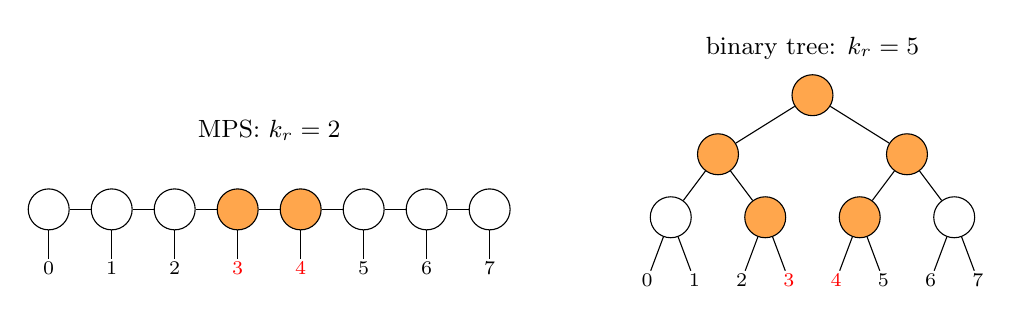
\begin{tikzpicture}[
  core/.style={circle,draw,minimum size=5.2mm,inner sep=0pt},
  hot/.style={core,fill=orange!70},
  st/.style={font=\scriptsize,inner sep=1pt},
  dif/.style={st,text=red,font=\scriptsize\bfseries}]
\node[font=\small] at (2.8,1.0) {MPS: $k_r=2$};
\foreach \i in {0,...,7} {
  \ifnum\i=3 \node[hot] (m\i) at (0.8*\i,0) {};
  \else\ifnum\i=4 \node[hot] (m\i) at (0.8*\i,0) {};
  \else \node[core] (m\i) at (0.8*\i,0) {}; \fi\fi
}
\foreach \i in {0,1,2,5,6,7} { \node[st] (y\i) at (0.8*\i,-0.75) {$\i$}; \draw (m\i) -- (y\i); }
\foreach \i in {3,4} { \node[dif] (y\i) at (0.8*\i,-0.75) {$\i$}; \draw (m\i) -- (y\i); }
\foreach \i [evaluate=\i as \j using int(\i+1)] in {0,...,6} { \draw (m\i) -- (m\j); }
\begin{scope}[xshift=7.6cm,yshift=-0.9cm]
\node[font=\small] at (2.1,2.95) {binary tree: $k_r=5$};
\foreach \i in {0,...,7} {
  \ifnum\i=3 \node[dif] (b\i) at (0.6*\i,0) {$\i$};
  \else\ifnum\i=4 \node[dif] (b\i) at (0.6*\i,0) {$\i$};
  \else \node[st] (b\i) at (0.6*\i,0) {$\i$}; \fi\fi
}
\node[core] (A0) at (0.3,0.8) {}; \node[hot] (A1) at (1.5,0.8) {};
\node[hot]  (A2) at (2.7,0.8) {}; \node[core] (A3) at (3.9,0.8) {};
\node[hot] (B0) at (0.9,1.6) {}; \node[hot] (B1) at (3.3,1.6) {};
\node[hot] (Rt) at (2.1,2.35) {};
\draw (b0)--(A0) (b1)--(A0) (b2)--(A1) (b3)--(A1) (b4)--(A2) (b5)--(A2) (b6)--(A3) (b7)--(A3);
\draw (A0)--(B0) (A1)--(B0) (A2)--(B1) (A3)--(B1) (B0)--(Rt) (B1)--(Rt);
\end{scope}
\end{tikzpicture}
\caption{Learned component $\pi_j=00000000$, unlearned $\pi_r=00011000$. They differ at sites $3$ and $4$ (red).
Orange: the Steiner subtree $\St(V_r)$. On the MPS the two sites are on adjacent cores ($k_r=2$); on the binary
tree the subtree passes through the root ($k_r=5$); on the HT tree $k_r=7$.}
\label{fig:steiner}
\end{figure}

\section{Two ways to decrease the loss}\label{sec:mechanisms}

Before stating the theorem we describe the two kinds of perturbation that lower the loss at $\theta_S$. The
theorem says that nothing else does better.

\paragraph{New channel along a subtree.} An entry on an unused channel of edge $e$ is multiplied, in the
contraction, by the neighbouring core's entries on the same channel, which are zero at $\theta_S$. So it changes
$W$ only if the neighbour also uses that channel. A set of cores therefore changes $W$ through unused channels only
if it is connected and all its cores use them together; the change is then a product of one small entry per core.
To produce component $r$ in this way, the set must contain every core on which $\pi_r$ differs from $\pi_j$, hence
all of $\St(V_r)$. With entries of size $t$ on the $k_r$ cores of $\St(V_r)$,
\begin{equation}\label{eq:route}
L-L_S=-c_r\,t^{k_r}+O(t^{2k_r}),\qquad c_r=s_r\,s_j^{(K-k_r)/K}
\end{equation}
(Proposition~\ref{prop:route}, at $a_v=s_j^{1/K}$). So the order is at most $k^*$.

\paragraph{Combining two cheaper perturbations.} A perturbation can also change the indices of $W$ on a set
$B$ of cores at lower cost, in two ways:
\begin{itemize}
\item if $B=\{v\}$ is a single core, by rotating its vector $q_v$ toward another basis vector, keeping the used
channel; the change in $W$ is linear in the rotation angle;
\item if $\lvert B\rvert\ge2$, by a new channel along $\St(B)$ as above; the change in $W$ has size $\epsilon$ when each
of the $\lvert\St(B)\rvert$ entries has size $\epsilon^{1/\lvert\St(B)\rvert}$.
\end{itemize}
Each such perturbation moves $W$ away from $s_jU_j$, which costs $\frac12s_j^2\epsilon^2$ at second order. Two of
them on disjoint core sets $B_1,B_2$ also produce, at second order, the product tensor with modified indices on
$B_1\cup B_2$. If that tensor is an unlearned component $r$, this gains $s_rs_j\epsilon_1\epsilon_2$. The net
change is a quadratic form in the amplitudes, which is negative in some direction iff the gains beat the costs.
The matrix below records the gains.

\begin{definition}[Coupling matrix]\label{def:coupling}
For $\ell\ge1$, let $\mathcal N_\ell$ be the set of pairs $(B,\beta)$, where $B$ is a nonempty set of cores with
$\lvert\St(B)\rvert\le\ell$ and $\beta$ assigns a basis index to each site of $B$ such that, on every core of $B$, the
indices differ from those of $\pi_j$. The coupling matrix $M_\ell$ is the symmetric matrix indexed by $\mathcal N_\ell$
with entries
\begin{equation}
M_\ell\big[(B_1,\beta_1),(B_2,\beta_2)\big]=\begin{cases}
s_r & \text{if }B_1\cap B_2=\emptyset\text{ and the string equal to }\beta_1\text{ on }B_1,\ \beta_2\text{ on }B_2,\\
 & \text{and }\pi_j\text{ elsewhere is }\pi_r\text{ for some component }r,\\
0 & \text{otherwise.}\end{cases}
\end{equation}
Let $\mu_\ell$ be its largest eigenvalue, and
\begin{equation}
\ell^*=\min\{\ell<k^*/2:\ \mu_\ell>s_j\}\qquad(\ell^*=\infty\text{ if there is no such }\ell).
\end{equation}
\end{definition}

$M_\ell$ has nonnegative entries, and $\mu_\ell$ is nondecreasing in $\ell$ because $M_\ell$ is a principal submatrix of
$M_{\ell+1}$. A nonzero entry requires a component $r$ with $V_r=B_1\sqcup B_2$, so if no component can be split into
two pieces with Steiner subtrees of at most $\ell$ cores, then $M_\ell=0$.

At level $\ell=1$ only single-core rotations occur. The corresponding block of the Hessian at $\theta_S$ (balanced,
$a_v=s_j^{1/K}$) is
\begin{equation}\label{eq:hessblock}
H_{\rm rot}=s_j^{(K-2)/K}\big(s_jI-M_1\big),
\end{equation}
so $\mu_1>s_j$ iff this block has a negative eigenvalue. For $\ell\ge2$ the combined perturbation has
$\lVert\theta-\theta_S\rVert\sim\epsilon^{1/\ell}$ and lowers the loss by $\sim\epsilon^2$, which is order $2\ell$ in the distance.

\section{Main result}

\begin{theorem}[Order of the saddle after one learned component]\label{thm:main}
Let $W^*$ be as in \eqref{eq:target} and $\theta_S$ as in \eqref{eq:saddle}, with $k^*\ge2$. Assume
\begin{enumerate}[label=(\alph*)]
\item $\mu_\ell\ne s_j$ for every $\ell<k^*/2$;
\item $\chi_e\ge2$ on the edges of $\St(V_r)$ for some $r$ with $k_r=k^*$; and, if $\ell^*<\infty$, there is a set
$X\subseteq\mathcal N_{\ell^*}$ such that the submatrix of $M_{\ell^*}$ on $X$ has largest eigenvalue above $s_j$ and every
edge $e$ has $\chi_e-1\ge\#\{(B,\beta)\in X:\lvert B\rvert\ge2,\ e\text{ is an edge of }\St(B)\}$.
\end{enumerate}
Then
\[
\ord(\theta_S)=\begin{cases}k^* & \text{if }\mu_\ell<s_j\text{ for all }\ell<k^*/2,\\
2\ell^* & \text{otherwise.}\end{cases}
\]
\end{theorem}

Assumption (a) excludes boundary cases. Assumption (b) provides the unused channels that the descent
perturbations of Section~\ref{sec:mechanisms} need. The theorem follows from three bounds, proved in
Section~\ref{sec:proofs}: $\ord\le k^*$ (Proposition~\ref{prop:route}), $\ord\ge\min(k^*,2\ell)$ whenever
$\mu_{\ell-1}<s_j$ (Proposition~\ref{prop:lower}), and $\ord\le2\ell$ whenever $\mu_\ell>s_j$ and $\ell<k^*/2$
(Proposition~\ref{prop:sharp}). The lower bound holds for any residual $\mathcal R$, not only sums of basis products.

\begin{corollary}\label{cor:cases}
Under the assumptions of Theorem~\ref{thm:main}:
\begin{enumerate}[label=(\roman*)]
\item If $k^*=2$, the saddle is strict.
\item If $k^*\in\{3,4\}$, the order is $k^*$ if $\mu_1<s_j$ and $2$ if $\mu_1>s_j$. So the order is $k^*$ unless the
Hessian has a negative eigenvalue.
\item If $W^*=s_jU_j+s_rU_r$ with $s_r<s_j$ (the larger component was learned), the order is $k_r$.
\item If $W^*=s_jU_j+s_rU_r$ with $s_r>s_j$, let $\ell_0=\min\max(\lvert\St(B_1)\rvert,\lvert\St(B_2)\rvert)$ over partitions
$V_r=B_1\sqcup B_2$. The order is $2\ell_0$ if $\ell_0<k_r/2$, and $k_r$ otherwise.
\item The order is below $k^*$ while the Hessian is positive semidefinite only if $k^*\ge5$.
\end{enumerate}
\end{corollary}

Part (iii) covers the typical situation in training, where components are learned in decreasing order of weight:
then the order is $k_r$, the size of a Steiner subtree, which depends on the tree.

\begin{example}[Order below $k^*$ with a positive semidefinite Hessian]\label{ex:pairstar}
MPS with six cores, $d=\chi=2$, learned $\pi_j=000000$ with $s_j=1$, and two unlearned components $\pi_1=110001$ and
$\pi_2=110010$ with weight $0.8$ each. Here $V_1=\{0,1,5\}$, so $k_1=6$, and $V_2=\{0,1,4\}$, so $k_2=5$; hence $k^*=5$.
No component differs from $\pi_j$ on exactly two cores, so $M_1=0$ and the Hessian is positive semidefinite. In
$M_2$, the pair $(\{0,1\},11)$ couples with $(\{5\},1)$ through component $1$ and with $(\{4\},1)$ through
component $2$, so $\mu_2\ge0.8\sqrt2\approx1.13>s_j$. Thus $\ell^*=2<k^*/2$ and the order is $4$. The descent uses a
new channel on cores $0,1$ that produces indices $11$ there (the string $110000$, not a component of $W^*$), together
with rotations of cores $4$ and $5$. Numerically, $\min_{\lVert\theta-\theta_S\rVert=t}L-L_S$ has slope $4.000$ in $t$ and
coefficient $-0.0350$, equal to the prediction $-(2\cdot0.8^2-1)/8$. With weights $0.6$, $\mu_2=0.85<1$ and the order is
$5$.
\end{example}

\section{Plateau lengths}

\begin{proposition}[Escape time; derived at leading order]\label{prop:escape}
Start gradient flow at $\theta_S$ plus a perturbation of size $\varepsilon$ along an order-$p$ descent direction of
Section~\ref{sec:mechanisms}. At leading order in $\varepsilon$, with the other variables relaxed to their
instantaneous minimum, the amplitude $b$ of the descent obeys $\dot b=c\,b^{p-1}$ with $c>0$, so the time to leave
the saddle is
\begin{equation}\label{eq:escape}
t_{\rm esc}\simeq\begin{cases}\ln(1/\varepsilon)/c, & p=2,\\[2pt] \varepsilon^{-(p-2)}/\big((p-2)\,c\big), & p\ge3.\end{cases}
\end{equation}
For a new channel along $\St(V_r)$ (equal entries), $p=k_r$ and $c=c_r=s_rs_j^{(K-k_r)/K}$.
\end{proposition}

In a run from small initialization of scale $\sigma$, the entries that will grow are of order $\sigma$ when the flow
reaches $\theta_S$, so the plateau there lasts $\propto\ln(1/\sigma)$ or $\propto\sigma^{-(p-2)}$. These entries already grow
somewhat while component $j$ is being learned. For $W^*=s_jU_j+s_rU_r$ with $s_r<s_j$, accounting for this growth
gives the time $\Delta t$ between learning $j$ and learning $r$:
\begin{equation}\label{eq:twocomp}
\Delta t\simeq\frac{1-s_r/s_j}{s_rs_j^{(K-2)/K}}\ln\frac1\sigma\quad(k_r=2),\qquad
\Delta t\simeq\frac{1-s_r/s_j}{(k_r-2)\,s_rs_j^{(K-k_r)/K}}\,\sigma^{-(k_r-2)}\quad(k_r\ge3),
\end{equation}
where the second formula assumes an initialization aligned with the target's basis vectors.

\paragraph{Evidence.}
\begin{itemize}
\item \emph{Order.} Minimizing $L-L_S$ numerically over spheres of radius $t$ in 32 cases (MPS, binary and HT trees,
$k^*$ from $2$ to $7$, including residuals that are not sums of basis products) gives slopes within $0.003$ of the
order predicted by Theorem~\ref{thm:main} in all 30 cases it covers; 12 further cases computed with independent code
agree to $5\cdot10^{-4}$.
\item \emph{Two components, $s_r<s_j$.} In about 11,600 gradient-flow runs on nine trees ($K$ from $3$ to $15$), the
fitted exponent of $\Delta t$ in $1/\sigma$ is $k_r-2$ for $k_r=3,4,5$, and for $k_r=6,7$ on two trees with
balanced initialization. For $k_r=2$ a logarithmic law fits better than a power law in all 14 settings, with slope
$0.98$--$1.01$ against the value $1$ predicted by \eqref{eq:twocomp}. On every edge outside $\St(V_r)$ the second
singular value of the corresponding matricization of $W$ stays below $4.3\,\sigma^2s_r$.
\item \emph{Order $2\ell^*<k^*$.} A pre-registered test (about 2,800 runs) started gradient flow at $\theta_S$ plus a
perturbation of size $\varepsilon$ and fitted $t_{\rm esc}\propto\varepsilon^{-\gamma}$. For $\varepsilon$ below the scale at
which the order-$2\ell^*$ descent is predicted to overtake the order-$k^*$ one, it found $\gamma=2.001\pm0.001$ for
$p=4$ ($k^*=5$ and $6$) and $\gamma=3.996$--$3.998$ for $p=6$ ($k^*=7$); the exponent $k^*-2$ fits $10^3$--$10^5$
times worse. Above that scale the results were mixed. This test has not been independently re-checked.
\end{itemize}

\section{Relation to prior work}\label{sec:prior}

\paragraph{Deep linear networks.} Saddle-to-saddle learning, the exponent $K-2$ and learning in order of decreasing
singular value are established for DLNs \citep{saxe2014exact,jacot2022saddletosaddle}. \citet[Thm~7]{achour2024loss}
show which DLN saddles are strict, a lower bound of the form ``order $\ge3$''. A binary tree with four sites is
exactly a depth-3 DLN; there $k^*=3$ and Theorem~\ref{thm:main} reduces to that classification.

\paragraph{Homogeneous models.} Near the origin the weights of a homogeneous model align with a critical direction of
the correlation with the target and escape after a time $\propto\sigma^{-(K-2)}$ \citep{kumar2025early}. If $1$, $2$ or
$k\ge3$ layers start small while the others are large, the escape takes time $O(1)$, $\propto\ln(1/\sigma)$ or
$\propto\sigma^{-(k-2)}$ \citep[Thm~4.2]{rawal2026theory}. Small weights keep the growth they acquired during earlier
plateaus \citep{kunin2025alternating,zhang2026saddletosaddle}, which is the factor $1-s_r/s_j$ in \eqref{eq:twocomp}.
These results take the number of small factors as given; Theorem~\ref{thm:main} determines it for TTNs.

\paragraph{The landscape of TTNs.} \citet{furman2026benign} analyse the landscape of the same model and loss. They
prove that local minima of minimum norm are global. At a minimum-norm critical point they consider the edges on which
the rank of the model is below that of the target. Each connected set of such edges, touching $n$ cores, gives a
straight-line perturbation along which the loss decreases at order $n$ (their Lemmas~D.8--D.9), an upper bound on the
order. They remark that with several separate such sets the smallest gives the fastest escape. They prove a lower bound
for one saddle (a parity target, their Prop.~5.3) and do not study the dynamics.

\paragraph{What is new.}
\begin{enumerate}[label=(\arabic*)]
\item A lower bound on the order at every saddle with one learned component, matching the upper bound, so the order is
determined exactly. Previously lower bounds were known only for DLNs and one parity saddle.
\item The order is set by the smallest single Steiner subtree $\St(V_r)$. For two components, the edges where the model
rank is below the target rank are exactly the edges of $\St(V_r)$, so the upper bound of \citet{furman2026benign} already
equals $k_r$ and the new part is the lower bound. With more components, those edges form the union of all the Steiner
subtrees, often the whole tree, while the order is set by the smallest one.
\item The case $\mu_\ell>s_j$: the order $2\ell^*$, and descent through index strings that are not components of the target.
\item The escape laws \eqref{eq:escape}--\eqref{eq:twocomp} for TTNs and their numerical tests.
\end{enumerate}

\section{Proofs}\label{sec:proofs}

Write $\varepsilon=\lVert\theta-\theta_S\rVert$, and let $\nu_v$ be the vector of entries of core $v$ on unused channels (entries
with at least one nonzero edge index).

\subsection{Decomposition by the cores on which a tensor differs from $U_j$}

Let $P_v=q_vq_v^\top$, $P_v^\perp=I-P_v$, and for a set $B$ of cores
\[
\Pi_B=\bigotimes_{v\in B}P_v^\perp\otimes\bigotimes_{v\notin B}P_v .
\]
The $2^K$ projections $\Pi_B$ are orthogonal and sum to the identity. Let $H_B$ be the range of $\Pi_B$: the tensors that
differ from $U_j$ exactly on the cores of $B$. A basis of $H_B$ is given by the products of basis vectors whose indices
differ from those of $\pi_j$ on every core of $B$, and $H_{B_1}\otimes H_{B_2}\cong H_{B_1\sqcup B_2}$ for disjoint sets.
Let $\mathcal R_B=\Pi_B\mathcal R$. By \eqref{eq:target},
\begin{equation}\label{eq:RB}
\mathcal R_B=\sum_{r:\,V_r=B}s_rU_r,\qquad\text{so}\qquad k^*=\min\{\lvert\St(B)\rvert:\mathcal R_B\ne0\}.
\end{equation}

\begin{lemma}\label{lem:decomp}
(i) $\theta_S$ is critical iff $\mathcal R_{\{v\}}=0$ for every core $v$, i.e.\ iff $k^*\ge2$.
(ii) Let $N(\theta)=\ip{U_j}{W(\theta)}$ and, for $B\ne\emptyset$, $m_B=\Pi_BW/N$. Wherever $N\ne0$,
\begin{equation}\label{eq:identity}
L(\theta)-L_S=\tfrac12(N-s_j)^2+\sum_{B\ne\emptyset}\Big[\tfrac{N^2}{2}\lVert m_B\rVert^2-N\ip{\mathcal R_B}{m_B}\Big].
\end{equation}
\end{lemma}
\begin{proof}
(i) Entries on unused channels do not change $W$ at first order (Section~\ref{sec:mechanisms}). A change of the used
entries of core $v$ changes $W$ within $H_\emptyset\oplus H_{\{v\}}$. So the gradient vanishes iff $\mathcal R$ has no
component in any $H_{\{v\}}$; its component in $H_\emptyset$ is zero because $\ip{U_j}{\mathcal R}=0$.
(ii) By orthogonality, $\lVert W-W^*\rVert^2=\sum_B\lVert\Pi_BW-\Pi_BW^*\rVert^2$, with $\Pi_\emptyset(W-W^*)=(N-s_j)U_j$, and for
$B\ne\emptyset$, $\Pi_BW^*=\mathcal R_B$ and $\Pi_BW=Nm_B$. Also $L_S=\frac12\sum_B\lVert\mathcal R_B\rVert^2$.
\end{proof}

\subsection{Upper bound $k^*$}

\begin{proposition}\label{prop:route}
Let $k_r=k^*$ and $\chi_e\ge2$ on the edges of $\St(V_r)$. At $a_v=s_j^{1/K}$, set the entry of each core $v\in\St(V_r)$
with physical index given by $\pi_r$ on the sites of $v$, index $1$ on the edges of $\St(V_r)$ and index $0$ on its other
edges, to $t$. Then $\lVert\theta(t)-\theta_S\rVert=\sqrt{k^*}\,t$ and
\[
L(\theta(t))-L_S=-s_r\,s_j^{(K-k^*)/K}\,t^{k^*}+\tfrac12s_j^{2(K-k^*)/K}\,t^{2k^*}.
\]
\end{proposition}
\begin{proof}
Expand the contraction by choosing, for each core of $\St(V_r)$, either its original entry or the new one. If a term
uses the new entry on one core of $\St(V_r)$ and the original entry on a neighbouring core of $\St(V_r)$, the shared
edge contracts index $1$ with index $0$ and the term vanishes. Only two terms remain: all original entries, giving
$s_jU_j$, and all new entries on $\St(V_r)$, giving $t^{k^*}s_j^{(K-k^*)/K}U$, where $U$ has the indices of $\pi_r$ on the
sites of $\St(V_r)$ and those of $\pi_j$ elsewhere. Since $\pi_r=\pi_j$ outside $V_r$, $U=U_r$. Hence
$W-W^*=-\mathcal R+t^{k^*}s_j^{(K-k^*)/K}U_r$, and $\ip{\mathcal R}{U_r}=s_r$.
\end{proof}

\subsection{Lower bound}

\paragraph{Cumulants.} Consider families $f=(f_B)_{B\subseteq V}$ with $f_B\in H_B$, with the product
$(f*g)_B=\sum_{B_1\sqcup B_2=B}f_{B_1}\otimes g_{B_2}$. This product is commutative and associative with unit
$(1,0,0,\dots)$, and every family with $f_\emptyset=0$ is nilpotent, so $\exp$ and $\log$ are finite sums and
$\log(f*g)=\log f+\log g$. With $m_\emptyset=1$, define $\kappa=\log m$. Explicitly,
\[
m_B=\sum_{\Pi\in\mathrm{Part}(B)}\ \bigotimes_{C\in\Pi}\kappa_C,\qquad
\kappa_B=\sum_{\Pi\in\mathrm{Part}(B)}(-1)^{\lvert\Pi\rvert-1}(\lvert\Pi\rvert-1)!\bigotimes_{C\in\Pi}m_C ,
\]
sums over set partitions of $B$. The $m_B$ and $\kappa_B$ are analytic near $\theta_S$ and vanish there for
$B\ne\emptyset$, so $\lVert\kappa_B\rVert\le C_0\varepsilon$.

\begin{lemma}\label{lem:locality}
For $\lvert B\rvert\ge2$, near $\theta_S$, $\lVert\kappa_B\rVert\le C_0\prod_{x\in\St(B)}\lVert\nu_x\rVert$. In particular
$\lVert\kappa_B\rVert\le C_0\varepsilon^{\lvert\St(B)\rvert}$.
\end{lemma}
\begin{proof}
Fix $x\in\St(B)$ and suppose $\nu_x=0$. Then all nonzero entries of $G_x$ have edge indices $0$, so $W$ factorizes at
$x$: $W=g_x\otimes\bigotimes_bW_b$, where $g_x$ is the physical vector of $G_x$, $b$ runs over the components of $T$ with
$x$ removed (node sets $V_b$), and $W_b$ is the contraction of component $b$ with its edge to $x$ set to $0$. The
projections $\Pi_B$ factorize core by core, so $m=m^{(x)}*\prod_bm^{(b)}$ with $m^{(x)}$ supported on $\{\emptyset,\{x\}\}$
and $m^{(b)}$ on subsets of $V_b$. Hence $\kappa=\log m^{(x)}+\sum_b\log m^{(b)}$ is supported on subsets of $\{x\}$ or of a
single $V_b$. $B$ is neither: if $x\in B$, then $B\not\subseteq\{x\}$ and $B\not\subseteq V_b$; if $x\notin B$ and
$B\subseteq V_b$, then the connected set $V_b$ contains $\St(B)$, which contains $x$. So $\kappa_B=0$ whenever $\nu_x=0$ for
some $x\in\St(B)$. In the power series of $\kappa_B$ around $\theta_S$, every monomial therefore contains a variable of
$\nu_x$ for each $x\in\St(B)$; factoring these out and bounding the rest on a small polydisc gives the claim.
\end{proof}

\begin{proposition}\label{prop:lower}
Let $\theta_S$ be critical and $2\le\ell\le\lceil k^*/2\rceil$. Let $S_{\ell-1}$ be the symmetric operator on
$\bigoplus_{\lvert\St(C)\rvert\le\ell-1}H_C$ with blocks $(x,y)\mapsto\ip{\mathcal R_{C_1\sqcup C_2}}{x\otimes y}$ for disjoint $C_1,C_2$ and
zero otherwise. If $\lambda_{\max}(S_{\ell-1})<s_j$, then $L(\theta)-L_S\ge-C\varepsilon^{\min(k^*,2\ell)}$ near $\theta_S$. In the
basis of products of basis vectors, $S_{\ell-1}=M_{\ell-1}$.
\end{proposition}
\begin{proof}
Let $p=\min(k^*,2\ell)$ and $y_C=\lVert\kappa_C\rVert$. Call $C$ \emph{small} if $\lvert\St(C)\rvert\le\ell-1$ and \emph{large}
otherwise. Then: (F1) a large set has $\lvert\St(C)\rvert\ge\ell\ge2$, so $y_C\le C_0\varepsilon^\ell$ by Lemma~\ref{lem:locality};
(F2) subsets of small sets are small; (F3) $\mathcal R_C=0$ for small $C$, since $\lvert\St(C)\rvert<k^*$; (F4) summing
$\ip{\mathcal R_B}{\kappa_{C_1}\otimes\kappa_{C_2}}$ over all $B$ and all unordered partitions $B=C_1\sqcup C_2$ into small sets gives
$\frac12\ip{\kappa_{\rm s}}{S_{\ell-1}\kappa_{\rm s}}\le\frac12\lambda_{\max}(S_{\ell-1})\lVert\kappa_{\rm s}\rVert^2$, where $\kappa_{\rm s}$ collects the
cumulants of small sets.

\emph{Quadratic term of \eqref{eq:identity}.} For small $B$, $m_B-\kappa_B$ is a sum of products of at least two cumulants of
small sets (F2), each at most $C_0\varepsilon\,y_C$ for one factor $C$. So
$\sum_{B\text{ small}}\lVert m_B\rVert^2\ge(1-C_2\varepsilon)\lVert\kappa_{\rm s}\rVert^2$; the terms with large $B$ are nonnegative and dropped.

\emph{Linear term.} Only $B$ with $\mathcal R_B\ne0$ contribute, and they have $\lvert\St(B)\rvert\ge k^*$. Expanding $m_B$ over set
partitions: the single cumulant gives $O(\varepsilon^{k^*})$ (Lemma~\ref{lem:locality}); two small blocks give (F4); one small and
one large block give at most $\frac\gamma2y_{C_1}^2+C_\gamma\varepsilon^{2\ell}$ (Young's inequality and F1); two large blocks give
$O(\varepsilon^{2\ell})$; three or more blocks give $O(\varepsilon)(y_{C_1}^2+y_{C_2}^2)$ if two blocks are small and $O(\varepsilon^{2\ell})$ otherwise.
Summing, $\sum_B\ip{\mathcal R_B}{m_B}\le\frac12(\lambda_{\max}(S_{\ell-1})+M\gamma+C\varepsilon)\lVert\kappa_{\rm s}\rVert^2+C_\gamma\varepsilon^p$.

\emph{Conclusion.} By \eqref{eq:identity}, dropping $\frac12(N-s_j)^2$,
$L-L_S\ge\frac N2[N(1-C_2\varepsilon)-\lambda_{\max}(S_{\ell-1})-M\gamma-C\varepsilon]\lVert\kappa_{\rm s}\rVert^2-NC_\gamma\varepsilon^p$. With
$g=s_j-\lambda_{\max}(S_{\ell-1})>0$, $\gamma=g/(4M)$ and $N\ge s_j-C\varepsilon$, the bracket is positive for small $\varepsilon$, so
$L-L_S\ge-C\varepsilon^p$.
\end{proof}

\subsection{Upper bound $2\ell$}

\begin{proposition}\label{prop:sharp}
Let $\ell<k^*/2$ and let $X\subseteq\mathcal N_\ell$ satisfy assumption (b) of Theorem~\ref{thm:main} with $\ell$ in place of
$\ell^*$, with largest eigenvalue $\rho>s_j$ of $M_\ell$ restricted to $X$. Then some curve has
$\lVert\theta(t)-\theta_S\rVert\le t$ and $L(\theta(t))-L_S\le-ct^{2\ell}$.
\end{proposition}
\begin{proof}
Take $a_v=a=s_j^{1/K}$ and a unit eigenvector $x\ge0$ of $M_\ell|_X$ for $\rho$ (Perron--Frobenius). For $0<\eta\le1$:
\begin{itemize}
\item for $(\{v\},\beta)\in X$, set the entry of $G_v$ with physical index $\beta$ and all edge indices $0$ to $a\eta x_{(\{v\},\beta)}$
(a rotation of $q_v$);
\item for $n=(B,\beta)\in X$ with $\lvert B\rvert\ge2$, let $h=\lvert\St(B)\rvert\le\ell$. On every edge of $\St(B)$ choose an unused index not
chosen by any other such element of $X$ (possible by (b)). Give each core $u\in\St(B)$ the entry $a(\eta x_n)^{1/h}$ with
physical index $\beta$ (if $u\in B$) or that of $\pi_j$ (if $u\notin B$), the chosen indices on the edges of $\St(B)$, and $0$
on its other edges.
\end{itemize}
Then $\lVert\theta-\theta_S\rVert\le C\eta^{1/\ell}$. In a nonzero term of the contraction, every connected set of edges carrying
nonzero indices uses the entries of a single element $n$ and equals its $\St(B)$. So $W$ is a sum over collections of
elements of $X$ on disjoint cores, each contributing the factor $\eta x_n$ and changing the indices on its set $B$. In
particular $N=s_j$, and $m_B=\eta m_B^{(1)}+\eta^2m_B^{(2)}+O(\eta^3)$, where $m^{(1)}$ collects single elements and $m^{(2)}$ pairs.

\emph{Order $\eta$.} $\sum_B\lVert m^{(1)}_B\rVert^2=\lVert x\rVert^2=1$. No single element has $B=V_r$, since that would need
$\lvert\St(B)\rvert\ge k^*>\ell$; so $\sum_B\ip{\mathcal R_B}{m^{(1)}_B}=0$ by \eqref{eq:RB}.

\emph{Order $\eta^2$.} If $M_\ell[n_1,n_2]=s_r>0$, then $\St(B_1)$ and $\St(B_2)$ are disjoint: otherwise their union would be a
connected set containing $V_r$ with at most $2\ell-1<k^*$ cores. So every nonzero entry of $M_\ell|_X$ corresponds to a pair
on disjoint cores, and $\sum_B\ip{\mathcal R_B}{m^{(2)}_B}=\frac12x^\top M_\ell|_Xx=\frac\rho2$.

By \eqref{eq:identity} with $N=s_j$: $L-L_S=\frac{s_j^2}{2}\eta^2-\frac{s_j\rho}{2}\eta^2+O(\eta^3)=-\frac{s_j}{2}(\rho-s_j)\eta^2+O(\eta^3)$.
Set $\eta=(t/C)^\ell$.
\end{proof}

\subsection{Proof of Theorem~\ref{thm:main} and Corollary~\ref{cor:cases}}

If $k^*=2$, the curve of Proposition~\ref{prop:route} has order $2$, and every critical point has order at least $2$.
Let $k^*\ge3$.

\emph{All $\mu_\ell<s_j$.} Proposition~\ref{prop:lower} with $\ell=\lceil k^*/2\rceil$ (using $\mu_{\lceil k^*/2\rceil-1}<s_j$) gives
$\ord\ge k^*$, and Proposition~\ref{prop:route} gives $\ord\le k^*$.

\emph{Some $\mu_\ell>s_j$.} If $\ell^*=1$, Proposition~\ref{prop:sharp} gives $\ord\le2$, so $\ord=2$. If $\ell^*\ge2$, then
$\mu_{\ell^*-1}<s_j$ by minimality and (a), so Proposition~\ref{prop:lower} at $\ell=\ell^*$ gives $\ord\ge2\ell^*$, and
Proposition~\ref{prop:sharp} gives $\ord\le2\ell^*$. \qed

\emph{Corollary.} (i) There is no $\ell<1$. (ii) The only level below $k^*/2$ is $\ell=1$. For \eqref{eq:hessblock}: rotating $q_u$ by
$\epsilon_u$ toward another basis vector changes $W$ by an orthonormal tensor times $a^{K-1}\epsilon_u$, and two rotations on cores
$u,v$ couple through any component with $V_r=\{u,v\}$ with coefficient $-s_ra^{K-2}$. So the block is
$a^{2(K-1)}I-a^{K-2}M_1=s_j^{(K-2)/K}(s_jI-M_1)$. (iii) With one unlearned component, each row of $M_\ell$ has at most one
nonzero entry, $s_r$, so $\mu_\ell\le s_r<s_j$. (iv) Same, with $\mu_\ell=s_r>s_j$ from the first $\ell$ that admits a partition,
namely $\ell_0$. (v) For $k^*\le4$, an order below $k^*$ requires $\mu_1>s_j$, which makes the Hessian indefinite. \qed

\subsection{Escape time (Proposition~\ref{prop:escape})}

\emph{New channel along $\St(V_r)$.} With the other entries fixed at $\theta_S$ and amplitudes $b_v$ on the cores of $\St(V_r)$,
Proposition~\ref{prop:route} gives $\dot b_v=A\prod_{u\ne v}b_u(s_r-A\prod_ub_u)$ with $A=a^{K-k_r}$. For equal small amplitudes,
$\dot b=s_rAb^{k_r-1}$, and $\frac{d}{dt}b^{-(p-2)}=-(p-2)c$ gives \eqref{eq:escape}.

\emph{Combined perturbation.} With one element of size $\lvert B\rvert\ge2$ (as in Example~\ref{ex:pairstar}), the rotations have $O(1)$
curvature and follow the amplitude $y=\prod_{v\in\St(B)}b_v$. Minimizing over them leaves $L-L_S\approx-\frac c2y^2$ with $c>0$
(in Example~\ref{ex:pairstar}, $c=0.8^2+0.8^2-1$). Then $\dot b_v=c\,b_v\prod_{u\ne v}b_u^2$, and for equal amplitudes
$\dot b=cb^{2\ell-1}$.

\emph{Growth before the plateau.} While $j$ is learned from aligned initialization, its cores grow as $\dot a\simeq s_ja^{K-1}$ and
the entries on $\St(V_r)$ already grow at rate $s_ra^{K-k_r}b^{k_r-1}$. For $k_r\ge3$,
$b^{-(k_r-2)}$ decreases by $(k_r-2)s_r\int a^{K-k_r}dt=(k_r-2)s_r\int a^{1-k_r}da/s_j=\frac{s_r}{s_j}\sigma^{-(k_r-2)}+O(1)$, so at the
plateau $b^{-(k_r-2)}=(1-s_r/s_j)\sigma^{-(k_r-2)}+O(1)$. For $k_r=2$, $\ln b$ grows by $\frac{s_r}{s_j}\ln\frac1\sigma+O(1)$. Inserting
into \eqref{eq:escape} gives \eqref{eq:twocomp}.

\section{Scope}
The theorem covers saddles with one learned component, targets that are sums of products of basis vectors (the lower
bound holds for any target), whitened inputs and the population loss. Saddles with several learned components and the
boundary cases $\mu_\ell=s_j$ are open. Proposition~\ref{prop:escape} is a leading-order derivation, not a theorem. When
$2\ell^*<k^*$ both kinds of perturbation are present, and the lower order wins only below a scale set by their
coefficients.

\bibliographystyle{plainnat}
\bibliography{references}
\end{document}
